%************************************************
\chapter{Outlook: Can pairs stabilize time crystalline dynamics?}
\label{ch:rydberg-timecrystal}

In this chapter, we revisit the model discussed in \autoref{ch:pair-localization-transition} and explore the question whether this form of disorder can sustain a time crystalline phase. The concrete protocol we study is similar to the previous chapter: After some interaction period $\tau$, all spins are flipped around the $x$-axis with angle $\phi=\pi(1-\epsilon)$. Hence, the Floquet unitary is given by:
\begin{equation}
	U_F = \exp\left[-i\pi(1-\epsilon)\sum_i S_x^{(i)}\right]\exp(-i\tau H_{XX})
\end{equation}
The dynamics are initialized in a $z$-polarized state $\ket{\psi_0} = \ket{\uparrow\ldots\uparrow}$ and the observable tracked is the total $z$-magnetization $M_z = N^{-1} \sum_i S_z^{(i)}$.

\begin{figure}[htb]
	\centering
	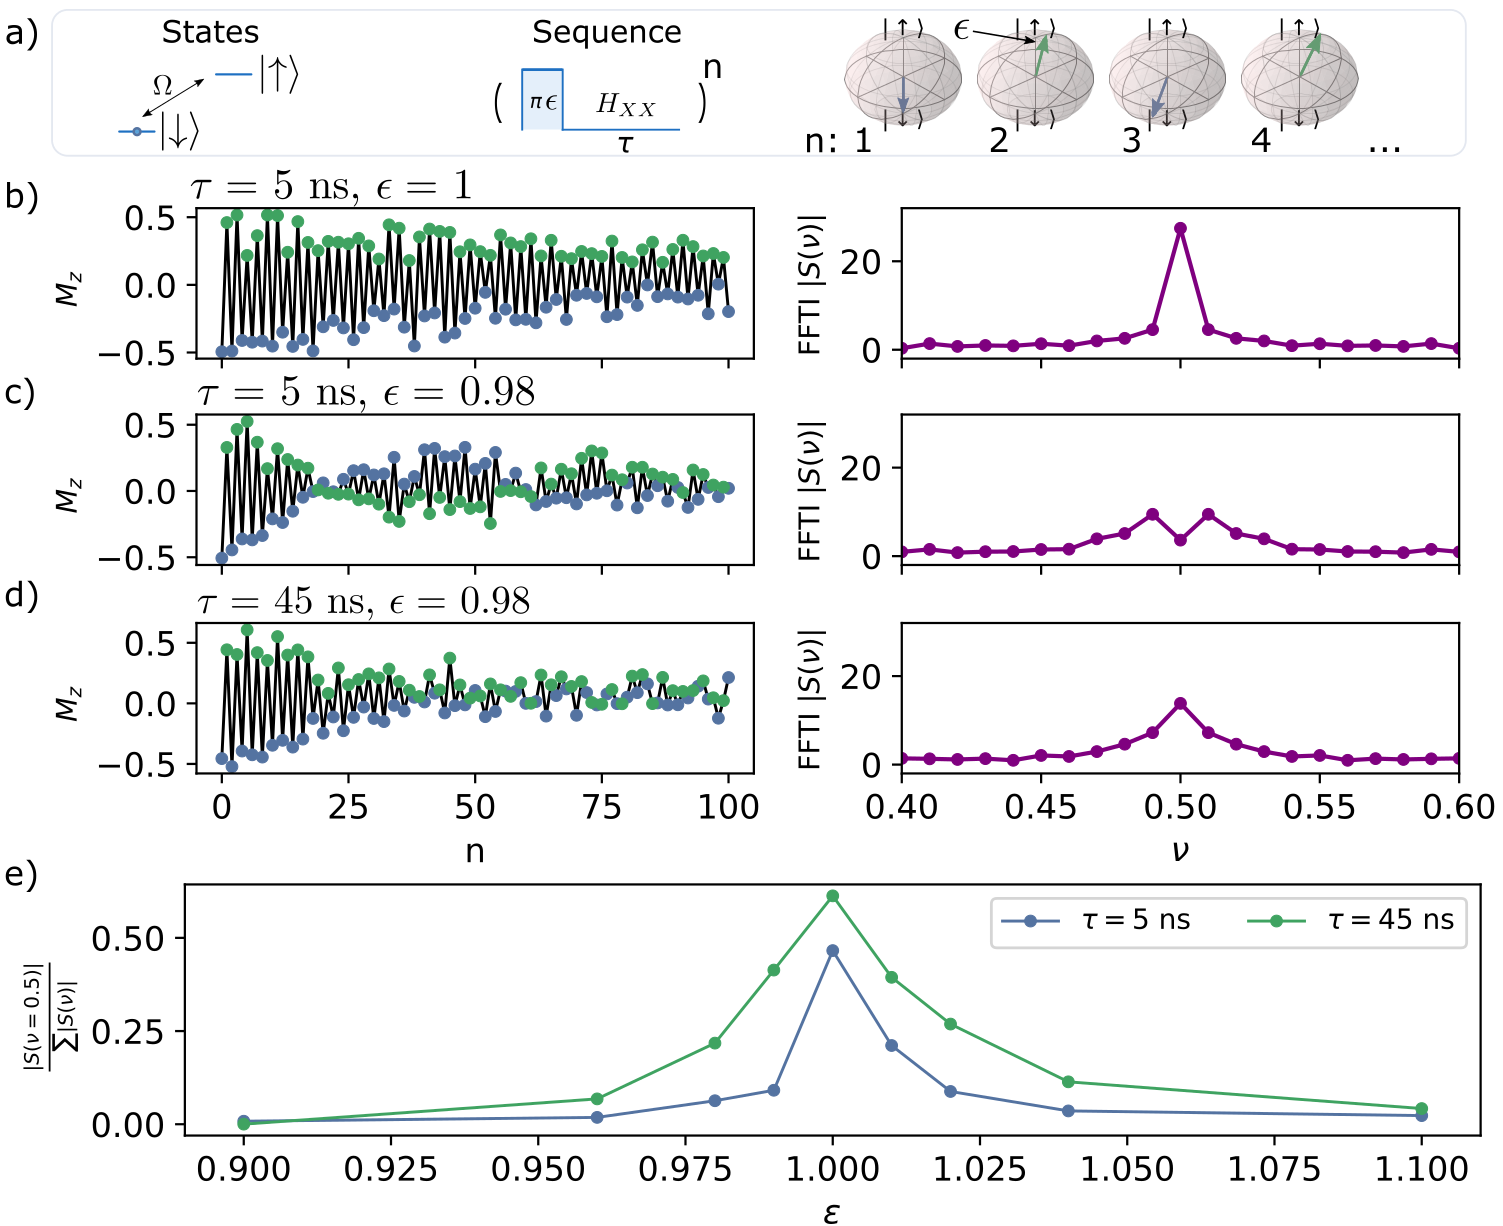
\includegraphics[width=\textwidth]{gfx/preliminary-timecrystal.png}
	\caption{Preliminary experimental results on time-crystalline signatures in a spatially disordered XX model. a) sketches the experimental sequence. Then experimental results for perfect rotation (b), short interaction times and imperfect rotation (c) and longer interaction times with imperfect rotation (d) follow. Left column depict the magnetization's time trace, while right column shows the Fourier transform of the signal. e) Then plots the normalized Fourier weight at $\nu=0.5$ versus rotational deviation $\epsilon$. Taken with permission from Ref.~\cite{geierShapingHamiltonianManybody}}
	\label{fig:rydberg-timecrystal-experiment}
\end{figure}

Preliminary experimental results of this protocol published in~\cite{geierShapingHamiltonianManybody} indicate that interactions indeed stabilize the magnetization dynamics (cf. \autoref{fig:rydberg-timecrystal-experiment})\footnote{Note that the graphic uses a different definition for the rotation angle. It uses $\phi=\epsilon \pi$ and thus $\epsilon = 1$ means perfect flips. In contrast, this thesis uses $\phi=(1-\epsilon)\pi$ with $\epsilon=0$ corresponding to perfect flips.}. Running the experiment with a rather short wait time of $\tau_1=5\mathrm{ns}$ finds period doubling for $\epsilon=0$ [cf. \autoref{fig:rydberg-timecrystal-experiment}(b) left] as expected due to symmetry. However, this signature is not stable to perturbations of the drive as increasing the drives deviation to $\epsilon=2\%$ replaces the stable period-doubled oscillations by a beating signal [cf. \autoref{fig:rydberg-timecrystal-experiment}(c) left]. 
However, increasing the wait time to $\tau_2=45$ns [cf. \autoref{fig:rydberg-timecrystal-experiment}(d) left] clearly reconstitutes the time crystalline signature. This is reflected by the so-called crystalline fraction [cf. \autoref{fig:rydberg-timecrystal-experiment}(b-d) right], which is defined as the normalized Fourier weight at $\nu=1/2$~\cite{choiObservationDiscreteTimecrystalline2017}. A systematic parameter sweep shows that increasing the interaction time $\tau$ not only leads to a larger crystalline fraction but also extends the range of $\epsilon$ where time crystalline behavior can be observed [cf. \autoref{fig:rydberg-timecrystal-experiment}(e)]. Thus, there is a clear stabilization effect due to the interactions which could imply the system to enter a time crystalline phase.


\section{Time crystal protocol with pairs}

In the following, we use the pair model to derive the functional form of the envelope of $|M_z(n)|$. The first obvious step is to just apply the pair model to solve the dynamics. So replacing $H_{XX}\rightarrow \sum_{\langle i,j\rangle}H_{pair}^{(i,j)}$, we find that $U_{F}$ factorizes completely between pairs:
\begin{align}
	U_F &\approx \sum_{\langle i,j\rangle} \exp\left[-i(1-\epsilon)\pi (S_x^i+S_x^j)\right] \exp\left[-i\tau H_{pair}^{(i,j)} \right] \equiv \sum_{\langle i,j\rangle} U_{F,pair}^{(i,j)}.\\
	\braket[1]{M_z}(n) &= \frac{1}{N}\sum_{\langle i,j\rangle} \braket[3]{\uparrow\uparrow}{(U_{F,pair}^{(i,j)\dagger})^n (S_z^{(i)}+S_z^{(j)})(U_{F,pair}^{(i,j)})^n}{\uparrow\uparrow} \equiv \frac{1}{N}\sum_{\langle i,j\rangle} \braket[1]{M^{(i,j)}_{z,pair}(n)}
\end{align}

Now we can exploit that $U_{F,pair}^{(i,j)}$ commutes with $S_x^{(i)}S_x^{(j)}$ to decompose the 4-dimensional Hilbertspace of each pair into two 2-dimensional subspaces. Thus, we can compute the exponential $U_{F,pair}^n$ analytically and find:
\begin{align}
	2\braket[1]{M^{(i,j)}_{z,pair}(n)} &\approx 2\cos(n\bar{J})\cos{n\theta} +
		2\sin(n\bar{J})\sin(n\theta)\underbrace{\frac{\sin\tau\cos\phi}{\sin\theta}}_{\equiv f}\\
	&= (1+f)\cos\left[ n(\bar{J}-\theta)\right] + (1-f)\cos\left[ n(\bar{J}+\theta)\right]\label{eq:pair-timecrystal-exact-solution}
\end{align}
where $\bar{J}=\frac{J\tau}{4}$ and $\cos\theta = \cos\bar{J}\cos\phi$.

To find the shape of the envelope, we assume $\epsilon\ll 1$ which is equivalent to $\phi \ll 1$ in a toggling frame where we swap the orientation of the $z$-axis in every step. Furthermore, we will consider only pairs where the interaction is stronger than the driving, i.e $\bar{J}>\phi$. The other pairs with $\bar{J}<\phi$ essentially oscillate around the $x$-axis with some deviation and thus dephase slowly among themselves on a timescale $\propto \epsilon$.
For the interaction dominated pairs, we can neglect the second term of \autoref{eq:pair-timecrystal-exact-solution} since its coefficient $(1-f)$ gets rather small because
\begin{equation}
	f = \frac{\sin\bar{J}\cos\phi}{\sqrt{1-\cos^2\bar{J}\cos^2\phi}}\approx \frac{\cos\phi}{\sqrt{1-\frac{\phi^2}{\sin^2\bar{J}}}}\approx 1+\frac{1}{2}\phi^2\left(\frac{1}{\sin^2\bar{J}}-1\right) \approx 1.
\end{equation}
Additionally, we can approximate $\theta$ for $\bar{J}<\pi$ as
\begin{equation}
	\theta = \arccos(\cos\bar{J}\cos\phi) \approx \arccos(\cos\bar{J}(1-\frac{\phi^2}{2}))\approx \bar{J} -\frac{\phi^2}{2\tan\bar{J}},
\end{equation}
which further justifies neglecting the second term, since not only its amplitude is small but it also oscillates quickly and therefore it averages out when considering the dynamics on a longer timescale.
Putting these results together we find for the approximate magnetization dynamics of an interaction dominated pair:
\begin{align}\label{eq:mz-interaction-dominated}
	\braket[1]{S_z^1+S_z^2}(n) \approx \cos n(\bar{J}-\theta) \approx \cos(n\frac{\phi^2}{2\tan\bar{J}})
\end{align}
From \autoref{fig:pair-model-timecrystal}(c), we can see that this approximation (blue line) matches the exact data (gray) essentially exactly.

\begin{figure}%[htb]
	\centering
	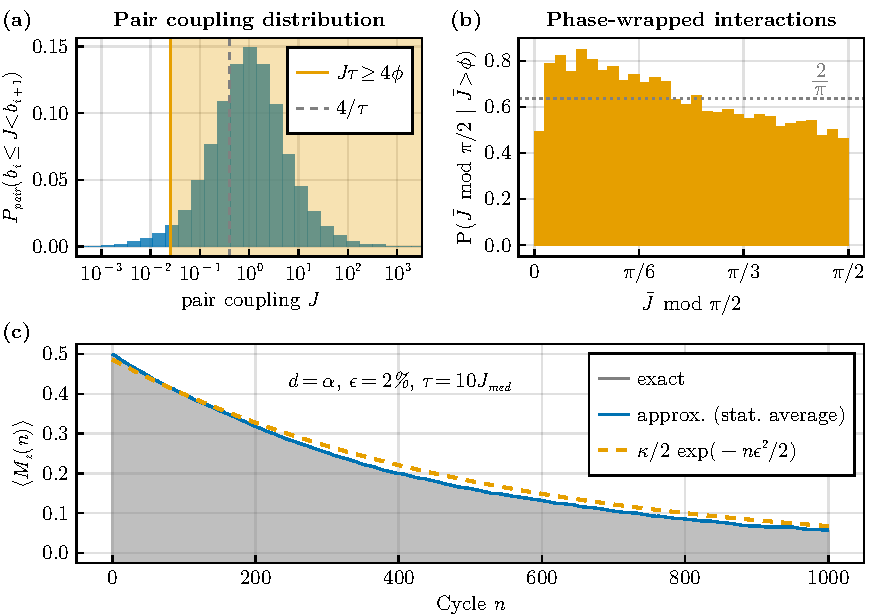
\includegraphics{gfx/part2/pair-model-timecrystal}
	\caption{Preliminary result of the pair model applied to the time crystal protocol for $d=\alpha$, $\epsilon=2\%$ and $\tau=10J_{med}$. (a) shows the distribution of the pair couplings as given by \autoref{eq:P-pair-J}. The yellow shaded area indicates the region where the approximation is applied. The gray, dashed, line indicates where $\bar{J}=1$ and thus phase wrapping sets in. (b) Resulting distribution if the couplings contained in the yellow area of panel (a) are phase wrapped. The gray, dotted, line is a guide to the eye and marks a uniform distribution. (c) Compares the time traces resulting from averaging exact pair dynamics (gray), averaging the approximated pair dynamics and (blue) and the approximate analytical average (yellow dashed).
	}
	\label{fig:pair-model-timecrystal}
\end{figure}


In principle, we now need to average this expression (\autoref{eq:mz-interaction-dominated}) over the appropriate part of the pair coupling distribution $P_{pair}(J)\mathrm{d}J$ (cf. \autoref{eq:P-pair-J}). This is analytically infeasible. Instead, we can exploit that this distribution is very broad (cf. \autoref{fig:pair-model-timecrystal}(a)), which leads to \emph{phase-wrapping}. This is the curious property of Floquet systems that their coupling are confined to a circle and strong coupling then just "wrap around".  Another way this manifests is the periodicity of \autoref{eq:mz-interaction-dominated} where any $\bar{J}$ can be mapped back to the interval $[0,\pi/2)$. Since the coupling distribution is so broad that most couplings wrap around multiple times, the distribution thus becomes effectively uniform (cf. \autoref{fig:pair-model-timecrystal}(b)). Exploiting this fact, we can approximate the average:
\begin{align}
	\braket[1]{M_z(n)} &= \frac{1}{2}\int_{4\phi/\tau}^\infty\!\mathrm{d}J P_{pair}(J) \braket[1]{S_z^1+S_z^2}(n) \\
	&\approx \frac{1}{2} \kappa \frac{2}{\pi}\int_{0}^{\pi/2} \mathrm{d}\bar{J} \braket[1]{S_z^1+S_z^2}(n) \\
%	&= \frac{1}{2} \kappa \frac{2}{\pi}\int_0^{\pi/2}\!\mathrm{d}\bar{J}\ \cos(n\frac{\phi^2}{2\tan\bar{J}})\\
	&= \frac{1}{2} \kappa \exp\left(-n\frac{\phi^2}2\right)
\end{align}
Here $\kappa=\int_{4\phi/\tau}^{\infty}\!\mathrm{d}JP_{pair}(J)$ denotes the fraction of pairs that are dominated by their interaction. \autoref{fig:pair-model-timecrystal}(c) confirms this to be a reasonable approximation. The slight deviation likely stem from the fact that the effective, phase-wrapped, coupling distribution shows a systematic deviation from a uniform distribution. This is likely due to the assumption that all couplings $\bar{J}>\phi$ are subject to the phase-wrapping. However the pair coupling distribution shows a slight curve in the regime $\phi\leq\bar{J}\leq\pi$, which explains the slight emphasis on smaller phase-wrapped couplings\footnote{A uniform distribution with a logarithmic $x$-axis would appear as a linear slope since the height of the bin is proportional to its width.}.

\section{Discussion}
The first-order pair model predicts a stabilization effect due to interactions, which shifts the decay timescale from $\mathcal{O}(\epsilon)$ to $\mathcal{O}(\epsilon^2)$. However, this stabilization does not increase with system size, because the pairs do not interact among each other. Therefore, the time crystalline signature is only a transient effect according to the pair model. However, it is unclear whether this  model captures the relevant physics of the situation. One way to check this is by experiment of course, where one could try to confirm the scaling of the decay timescale $\tau_{decay}\propto\epsilon^2$ and perform more extensive numerical checks in small systems.

From the theoretical side, there are some more possible mechanisms that could stabilize the time crystalline signature. For one, the Rydberg spins also generate some on-site potential due to van der Waals interactions, which were neglected so far. This term can be combined with the driving field to effectively slight deviations in the rotation axis. As we have seen in the previous \autoref{ch:metronome-spin}, such a spatially dependent drive can have a huge influence on the lifetime of the system. However, since this does not cause further interactions between pairs and thus the dynamics stay constricted to small Hilbert spaces, it is unlikely that this effect would have a large impact in this scenario.

A likely more fruitful approach is to incorporate pair-pair interactions. For an XXZ model, we derived (cf. \autoref{ch:pair-localization-transition}) that these pair-pair interactions are effectively a kind of Ising model of pairs. Since disordered Ising models are known to feature time crystalline phases, we deem this avenue quite promising to study. Unfortunately, these terms thwart the integrability and so one will need to resort to numerics or find some other clever approach to tackle this problem analytically.
The extension of this idea to XX models is also not straight-forward as it requires a better understanding of the next order of perturbation theory, which was already discussed previously in \autoref{ch:discussion-pair-localization}.

While we could not confirm the presence of time crystal in this preliminary analysis of the pair model, we also dit not rule it out. However, just the base pair description does not lend itself to produce a stable time crystal. Hence, new insights beyond bare pairs are required to draw a definitive conclusion on this matter.

